\documentclass{article}
\usepackage{mathrsfs}
\usepackage{amsmath}
\usepackage{amsthm}
\usepackage{amssymb}
\usepackage{graphicx}
\usepackage{color}
\DeclareMathOperator*{\argmin}{argmin}
%\include{macros}
%\usepackage{floatflt}
%\usepackage{graphics}
%\usepackage{epsfig}


\theoremstyle{definition}
\newtheorem{theorem}{Theorem}[section]
\newtheorem{lemma}[theorem]{Lemma}
\newtheorem{proposition}[theorem]{Proposition}
\newtheorem{corollary}[theorem]{Corollary}

\theoremstyle{definition}
\newtheorem*{defition}{Definition}
\newtheorem*{example}{Example}

\theoremstyle{remark}
\newtheorem*{remark}{Remark}
\newtheorem*{note}{Note}
\newtheorem*{exercise}{Exercise}

\setlength{\oddsidemargin}{-0.25 in}
\setlength{\evensidemargin}{-0.25 in} \setlength{\topmargin}{-0.25
in} \setlength{\textwidth}{7 in} \setlength{\textheight}{8.5 in}
\setlength{\headsep}{0.25 in} \setlength{\parindent}{0 in}
\setlength{\parskip}{0.1 in}

\newcommand{\homework}[4]{
\pagestyle{myheadings} \thispagestyle{plain}
\newpage
\setcounter{page}{1} \setcounter{section}{#4} \noindent
\begin{center}
\framebox{ \vbox{\vspace{2mm} \hbox to 6.28in { {\bf
THU-70250043,~Pattern~Recognition~(Spring 2016) \hfill Homework: 2} }
\vspace{6mm} \hbox to 6.28in { {\Large \hfill #1 \hfill} }
\vspace{6mm} \hbox to 6.28in { {\it Lecturer: #2 \hfill} }
\vspace{2mm} \hbox to 6.28in { {\it Student: #3 \hfill} }
\vspace{2mm} } }
\end{center}
\markboth{#1}{#1} \vspace*{4mm} }


\begin{document}

\homework{Parameter Estimation Method}{Changshui Zhang
\hspace{5mm} {\tt zcs@mail.tsinghua.edu.cn}}{Qingfu Wen (2015213495)\hspace{5mm} {\tt qingfu.wen@gmail.com
 } }{8}

%%%%%%%%%%%%%%%%%%%%%%%%%%%%%%%%%%%%%%%%%%%%%%%%%%%%%%%%%%%%%%%%%%%%
% Section 2.  Problem
%%%%%%%%%%%%%%%%%%%%%%%%%%%%%%%%%%%%%%%%%%%%%%%%%%%%%%%%%%%%%%%%%%%%

\section*{}
1.
\begin{figure}[htbp]
  \centering
  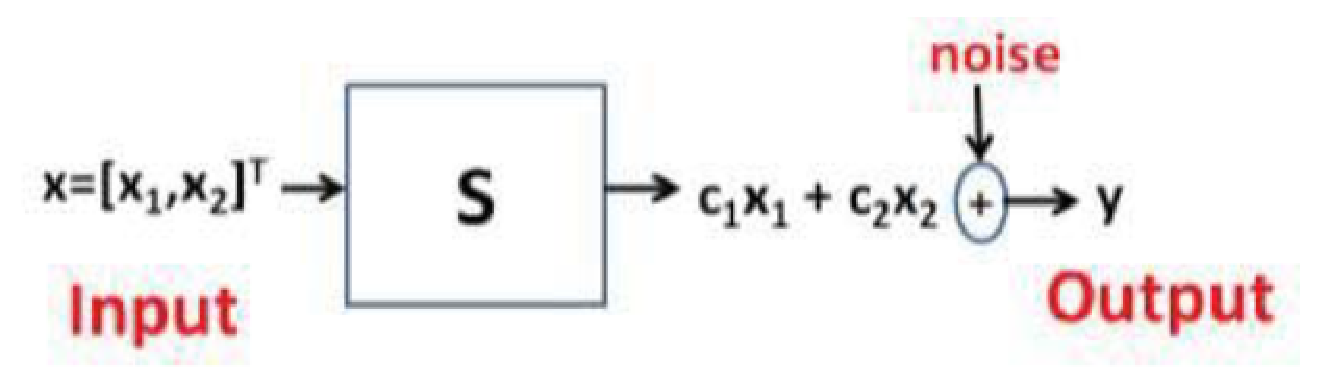
\includegraphics[width=0.35\textwidth]{figure1.eps}
  \caption{System S}\label{}
\end{figure}

 Figure 1 shows a system S which takes two inputs $x_1,x_2$(which are deterministic) and outputs a linear combination of those two inputs, $c_1x_1+c_2x_2$, introduces an additive error $\epsilon$ which is a random variable following some distribution. Thus the output $y$ that you observe is given by equation (1). Assume that you have $n>2$ instances $<x_{j1},x_{j2},y_j>_{j=1,...,n}$
$$y=c_1x_1+c_2x_2+\epsilon  \qquad (1)$$
In other words having n equations in your hand is equivalent to having n equations of the following form:$y_j=c_1x_{j1}+c_2x_{j2}+\epsilon _j,j=1,...,n $ The goal is to estimate $c_1,c_2$ from those measurements by maximizing conditional log-likelihood given the input, under different assumptions for the noise. Specifically:

1) Assume that the $\epsilon _i$ for $i=1,...,n$ are iid Gaussian random variables with zero mean and variance $\sigma ^2$.

\qquad (a) Find the conditional distribution of each $y_i$ given the inputs

\qquad \emph{\textbf{SOLUTION:}}

\qquad\qquad Since $y_j=c_1x_{j1}+c_2x_{j2}+\epsilon _j,j=1,...,n $, $y_j-c_1x_{j1}-c_2x_{j2}\sim N(0,\sigma^2)$.

\qquad\qquad Thus, $y_j\sim N(c_1x_{j1}+c_2x_{j2},\sigma^2)$.

\qquad (b) Compute the log-likelihood of $y$ given the inputs

\qquad \emph{\textbf{SOLUTION:}}

\qquad\qquad The PDF of $y_j$ is \[f(y_j)= \frac{1}{\sqrt{2\pi}\sigma}\exp\left(-\frac{(y_j-c_1x_{j1}-c_2x_{j2})^2}{2\sigma^2}\right)\]
\qquad\qquad the log-likelihood function is
\begin{equation}\nonumber
\begin{aligned}
l(c_1,c_2) &= \ln L(c_1,c_2)\\
           &= \ln \prod_{j=1}^{n} \frac{1}{\sqrt{2\pi}\sigma}\exp\left(-\frac{(y_j-c_1x_{j1}-c_2x_{j2})^2}{2\sigma^2}\right)\\
           &= \frac{n\ln(\sqrt{2\pi}\sigma)}{2\sigma^2}\sum_{j=1}^{n}(y_j-c_1x_{j1}-c_2x_{j2})^2
\end{aligned}
\end{equation}

\qquad (c) Maximize the likelihood above to get $c_{ls}$

\qquad \emph{\textbf{SOLUTION:}}

\begin{equation}\nonumber
\begin{aligned}
c_{ls} &= \mathop{\argmin}_{c}\sum_{j=1}^{n}(y_j-c_1x_{j1}-c_2x_{j2})^2 \\
\end{aligned}
\end{equation}
\qquad for $c_1$, we get
\begin{equation}\nonumber
\begin{aligned}
\frac{\partial\sum_{j=1}^{n}(y_j-c_1x_{j1}-c_2x_{j2})^2}{\partial c_1} &= 0\\
2c_1\sum_{j=1}^{n} x_{j1}^2 - 2\sum_{j=1}^{n}x_{j1}y_j &= 0\\
c_1 = \frac{\sum_{j=1}^{n}x_{j1}y_j}{\sum_{j=1}^{n} x_{j1}^2}
\end{aligned}
\end{equation}
\qquad similarly, we get
\[c_1 = \frac{\sum_{j=1}^{n}x_{j2}y_j}{\sum_{j=1}^{n} x_{j2}^2}\]
\qquad Let $y = [y_1, y_2,\cdots,y_n]^T$, $X$ be a $n*2$ matrix that $X_{ij}=x_{ij}$, $c=[c_1,c_2]^T$. Then
\[c = (X^TX)^{-1}X^Ty\]

2) Assume that the $\epsilon _i$ for $i=1,...,n$ are independent Gaussian random variables with zero mean and variance $Var(\epsilon _i)=\sigma _i$.

\qquad (a) Find the conditional distribution of each $y_i$ given the inputs

\qquad \emph{\textbf{SOLUTION:}}

\qquad\qquad $y_j\sim N(c_1x_{j1}+c_2x_{j2},\sigma_i^2)$.

\qquad (b) Compute the log-likelihood of $y$ given the inputs

\qquad \emph{\textbf{SOLUTION:}}

\qquad\qquad The PDF of $y_j$ is \[f(y_j)= \frac{1}{\sqrt{2\pi}\sigma_j}\exp\left(-\frac{(y_j-c_1x_{j1}-c_2x_{j2})^2}{2\sigma_j^2}\right)\]
\qquad\qquad the log-likelihood function is
\begin{equation}\nonumber
\begin{aligned}
l(c_1,c_2) &= \ln L(c_1,c_2)\\
           &= \ln \prod_{j=1}^{n} \frac{1}{\sqrt{2\pi}\sigma_j}\exp\left(-\frac{(y_j-c_1x_{j1}-c_2x_{j2})^2}{2\sigma_j^2}\right)\\
           &= \sum_{j=1}^{n}\ln(\sqrt{2\pi}\sigma_j)\sum_{j=1}^{n}\frac{(y_j-c_1x_{j1}-c_2x_{j2})^2}{2\sigma_j^2}
\end{aligned}
\end{equation}

\qquad (c) Maximize the likelihood above to get $c_{wls}$

\qquad \emph{\textbf{SOLUTION:}}

\qquad\qquad we need to minimize $||W(y-Xc)||$ that $W$ is a diagonal matrix, $W_{ii}=\frac{1}{\sigma_i}$. Similarly,$c_{wls} = (X^TW^TWX)^{-1}X^TW^TWy$

3) Assume that the $\epsilon _i$ for $i=1,...,n$ has density $f_{\epsilon_i}(x)=f(x)=\frac{1}{2b}exp(-\frac{|x|}{b})$. In other words our noise is iid following Laplace distribution with location parameter $\mu =0$ and scale parameter $b$.

\qquad (a) Find the conditional distribution of each $y_i$ given the inputs

\qquad \emph{\textbf{SOLUTION:}}

\qquad\qquad Since $y_j=c_1x_{j1}+c_2x_{j2}+\epsilon _j,j=1,...,n $, $\epsilon _j = y_j-c_1x_{j1}-c_2x_{j2}$.

\qquad\qquad Thus, the density function of $y_j$ is $f(y_j)=\frac{1}{2b}exp(-\frac{|y_j-c_1x_{j1}-c_2x_{j2}|}{b})$.
$y_j$ is a Laplace distribution with $\mu=c_1x_{j1}+c_2x_{j2}$ and scale parameter $b$.

\qquad (b) Compute the log-likelihood of $y$ given the inputs

\qquad \emph{\textbf{SOLUTION:}}

\qquad\qquad The PDF of $y_j$ is \[f(y_j)= \frac{1}{2b}exp(-\frac{|y_j-c_1x_{j1}-c_2x_{j2}|}{b})\]
\qquad\qquad the log-likelihood function is
\begin{equation}\nonumber
\begin{aligned}
l(c_1,c_2) &= \ln L(c_1,c_2)\\
           &= \ln \prod_{j=1}^{n} \frac{1}{2b}exp(-\frac{|y_j-c_1x_{j1}-c_2x_{j2}|}{b})\\
           &= \frac{n\ln(2b)}{b}\sum_{j=1}^{n}|y_j-c_1x_{j1}-c_2x_{j2}|
\end{aligned}
\end{equation}

\qquad (c) Comment on why this model leads to more robust solution.


2.  Consider a normal $p(x)\sim N(\mu,\sigma^2)$ and Parzen-window function $\phi(x)\sim N(0,1)$ Show that the Parzen-window estimate
$$
p_n(x) = \frac{1}{nh_n}\sum_{i=1}^{n}\phi(\frac{x-x_i}{h_n})
$$
has the following properties:

(a)$\overline{p}_n(x)\sim N(\mu,\sigma^2+h_n^2)$

\emph{\textbf{SOLUTION:}}\\
\begin{equation}\nonumber
\begin{aligned}
\overline{p}_n(x) &= E[p_n(x)] \\
&= E[\frac{1}{n}\sum_{i=1}^{n}\frac{1}{h_n}\phi(\frac{x-x_i}{h_n})]\\
&= \frac{1}{h_n}E[\phi(\frac{x-x_i}{h_n})]\\
&= \frac{1}{h_n}\int \phi(\frac{x-v}{h_n})p(v)dv \\
&= \frac{1}{h_n}\int h_n \frac{1}{\sqrt{2\pi}h_n}\exp(-\frac{(x-v)^2}{h_n^2})*\frac{1}{\sqrt{2\pi}\sigma}\exp(-\frac{(v-\mu)^2}{\sigma^2}) dv\\
&= N(x;\mu,\sigma^2+h_n^2)
\end{aligned}
\end{equation}
(b)$Var[p_n(x)] \simeq \frac{1}{2nh_n\sqrt{\pi}}p(x)$

\emph{\textbf{SOLUTION:}}\\
\begin{equation}\nonumber
\begin{aligned}
Var[p_n(x)] &= \frac{1}{n^2}\sum_{i=1}^{n}\left(\frac{1}{h_n^2}E(\phi^2(\frac{x-x_i}{h_n}))-E^2(p(x))\right)\\
&= \frac{1}{n}\left(\int N^2(x;v,h_n^2)N(v;\mu,\sigma^2)dv -E^2(p(x))\right)\\
&= \frac{1}{n}\left(\frac{1}{2h_n\sqrt{\pi}}N(x;\mu,\sigma+\frac{h_n^2}{2}) - \frac{1}{2\sqrt{(\sigma^2+h_n^2)\pi}}N(x;\mu,\frac{\sigma^2+h_n^2}{2})\right)\\
\end{aligned}
\end{equation}
When $h_n$ gets small, \[Var[p_n(x)] \simeq \frac{1}{2nh_n\sqrt{\pi}}p(x)\]

(c)$p(x)-\overline{p}_n(x)\simeq \frac{1}{2}(\frac{h_n}{\sigma})^2[1-(\frac{x-\mu}{\sigma})^2]p(x)$ for small $h_n $

(Note: if $h_n = \frac{h_1}{\sqrt n} $, this show that the error due to bias goes to zero as $1/n $ , whereas the
standard deviation of the noise only goes to zero as ${\sqrt[4]{n}} $.)

\emph{\textbf{SOLUTION:}}\\
\begin{equation}\nonumber
\begin{aligned}
p(x)-\overline{p}_n(x) &= N(x;\mu,\sigma^2)-N(x;\mu,sigma^2+h_n^2)\\
&= (1-\frac{N(x;\mu,\sigma^2)}{N(x;\mu,sigma^2+h_n^2)})N(x;\mu,h_n^2)\\
&= \left(1-\sqrt{\frac{\sigma^2}{\sigma^2+h_n^2}}\exp(\frac{h_n^2(x-\mu)^2}{2(\sigma^2+h_n^2)\sigma^2})\right)p(x)\\
\end{aligned}
\end{equation}
From Taylor series, when $h_n$ is very small,
\[\sqrt{\frac{\sigma^2}{\sigma^2+h_n^2}}=\sqrt{1-\frac{h_n^2}{\sigma^2+h_n^2}}\approx1-\frac{h_n^2}{2(\sigma^2+h_n^2)}\]
\[\exp(\frac{h_n^2(x-\mu)^2}{2(\sigma^2+h_n^2)\sigma^2}) \approx 1+\frac{h_n^2(x-\mu)^2}{2(\sigma^2+h_n^2)\sigma^2}\]
Thus
\begin{equation}\nonumber
\begin{aligned}
p(x)-\overline{p}_n(x) &\approx \left(1-(1-\frac{h_n^2}{2(\sigma^2+h_n^2)})(1+\frac{h_n^2(x-\mu)^2}{2(\sigma^2+h_n^2)\sigma^2}))\right)p(x)\\
&\approx \frac{h_n^2}{2\sigma^2}(1-\frac{(x-\mu)^2}{\mu^2})p(x)
\end{aligned}
\end{equation}
3.  One measure of the difference between two distributions in the same space is the
Kullback-Leibler divergence of Kullback-Leibler "distance":

$$
D_{KL}(p_1(x),p_2(x)) = \int p_1(x)ln\frac{p_1(x)}{p_2(x)}dx
$$


(This "distance" does not obey the requisite symmetry and triangle inequalities for a metric.)Suppose we seek to approximate an arbitrary distribution $p_2(x)$ by a normal $p_1(x)\sim N(\mu,\Sigma)$ .
Show that the values that lead to the smallest Kullback-Leibler divergence are the obvious ones:

$$
\mu = \epsilon_2[x]
$$
$$
\Sigma = \epsilon_2[(x-\mu)(x-\mu)^T]
$$

where the expectation $\epsilon_2$ taken is over the density $p_2(x)$.

\emph{\textbf{SOLUTION:}}\\
$p_1(x)\sim N(\mu,\Sigma)$, $p_2(x)$ is an arbitrary distribution. From $p_2(x)$, we can get KL divergence
\begin{equation}\nonumber
\begin{aligned}
D_{KL}(p_2(x),p_1(x)) &= \int p_2(x)ln\frac{p_2(x)}{p_1(x)}dx\\
 &= \int p_2(x)ln p_2(x)dx + \frac{1}{2}\int p_2(x)[\ln(2\pi)+\ln\Sigma+(x-\mu)^T\Sigma^{-1}(x-\mu)]dx
\end{aligned}
\end{equation}
To minimize $D_{KL}(p_2(x),p_1(x))$ with parameter $\mu, \Sigma$, set
\[\frac{\partial D_{KL}(p_2(x),p_1(x))}{\partial \mu}=-\int p_2(x)\Sigma^{-1}(x-\mu)dx=0\]
\[\frac{\partial D_{KL}(p_2(x),p_1(x))}{\partial \Sigma}=\int p_2(x)[\Sigma^{-1}-(x-\mu)^T\Sigma^{-2}(x-\mu)]dx=0\]
Then we get
\[\int p_2(x)(x-\mu)dx=0 \Rightarrow \epsilon_2(x-\mu) = 0\]
\[\int p_2(x)[\Sigma-(x-\mu)(x-\mu)^T]dx=0 \Rightarrow \epsilon_2(\Sigma-(x-\mu)(x-\mu)^T) = 0\]
Thus
\[\mu = \epsilon_2(x)\]
\[\Sigma = \epsilon_2[(x-\mu)(x-\mu)^T]\]
4. (Programming) Assume  $p(x)\sim0.1N(-1,1)+0.9N(1,1)$.  Draw n samples from $p(x)$, for example, $n=5,10,50,100,\cdots,1000,\cdots,10000$. Use Parzen-window method to estimate $p_n(x)\approx p(x)$ (Hint: use randn() function in matlab to draw samples)

(a) Try window-function $P(x)=\left\{
\begin{aligned}
&\frac{1}{a},-\frac{1}{2}a\leq x\leq \frac{1}{2}a \\
&0,otherwise.
\end{aligned}
\right.$. Estimate $p(x)$ with different window width $a$.

\begin{figure}[!htbp]
\begin{minipage}[t]{0.3\linewidth}
\centering
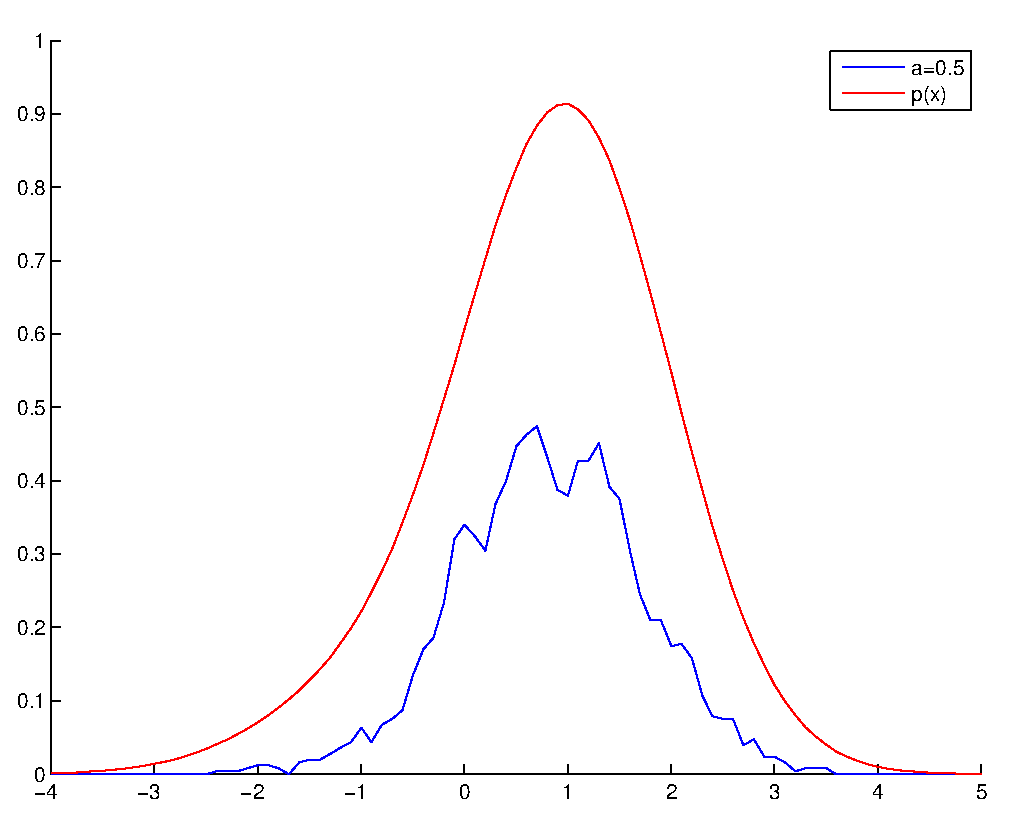
\includegraphics[width=2.1in]{0_5.eps}
\caption{a=0.5}
\end{minipage}%
\begin{minipage}[t]{0.3\linewidth}
\centering
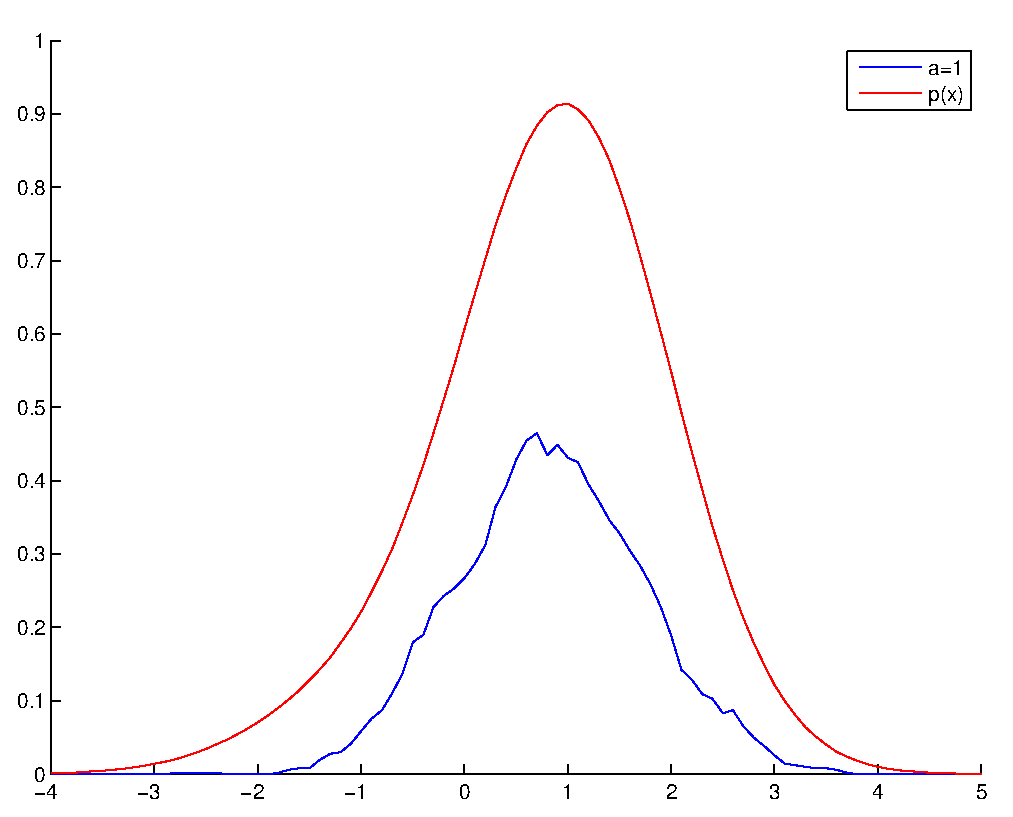
\includegraphics[width=2.1in]{1.eps}
\caption{a=1}
\end{minipage}
\begin{minipage}[t]{0.3\linewidth}
\centering
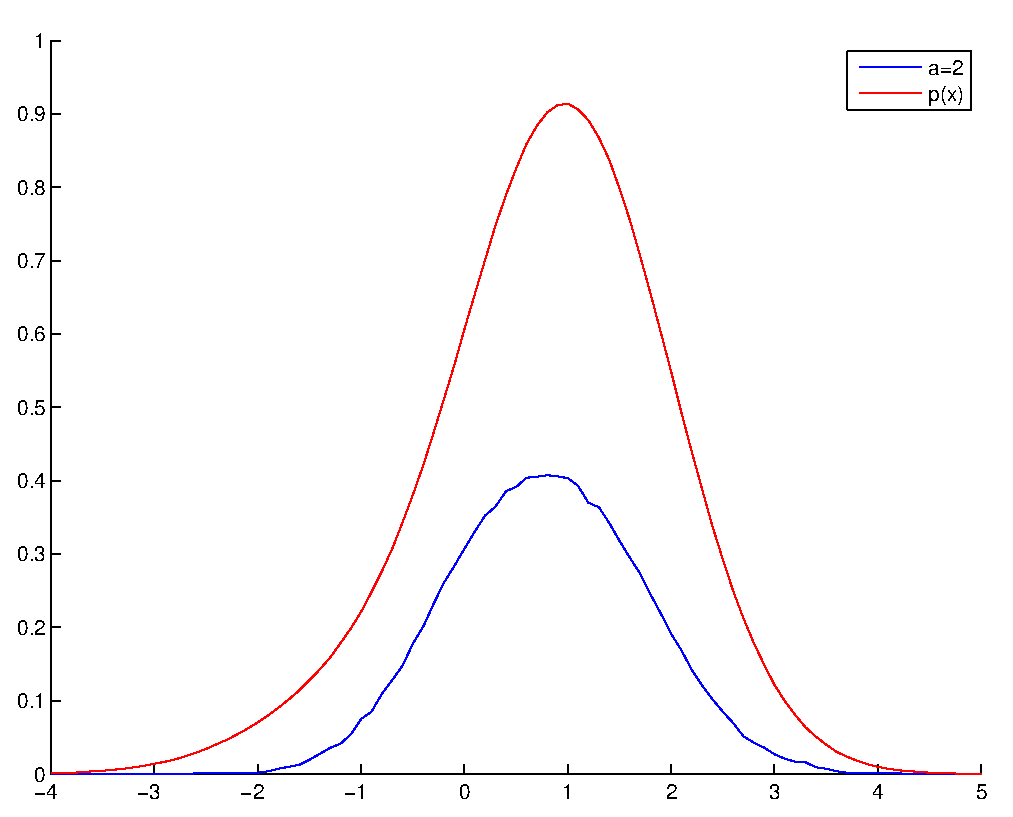
\includegraphics[width=2.1in]{2.eps}
\caption{a=2}
\end{minipage}
\end{figure}
\begin{figure}[!htbp]
\begin{minipage}[t]{0.3\linewidth}
\centering
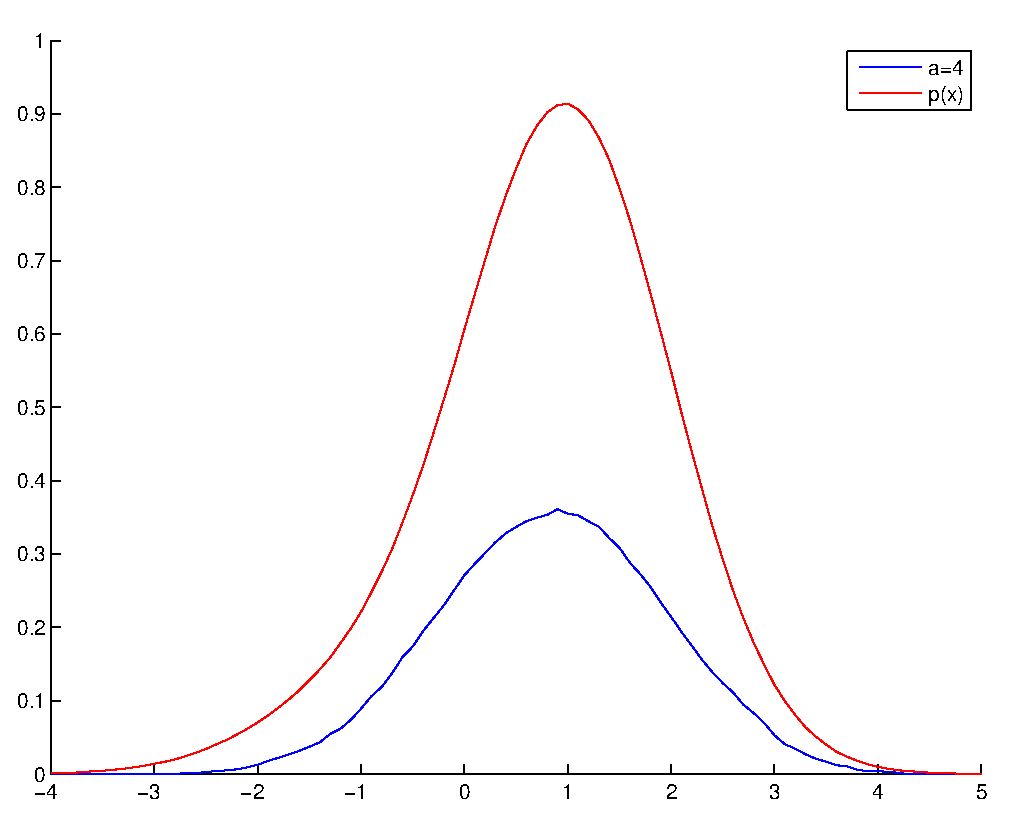
\includegraphics[width=2.1in]{4.eps}
\caption{a=4}
\end{minipage}%
\begin{minipage}[t]{0.3\linewidth}
\centering
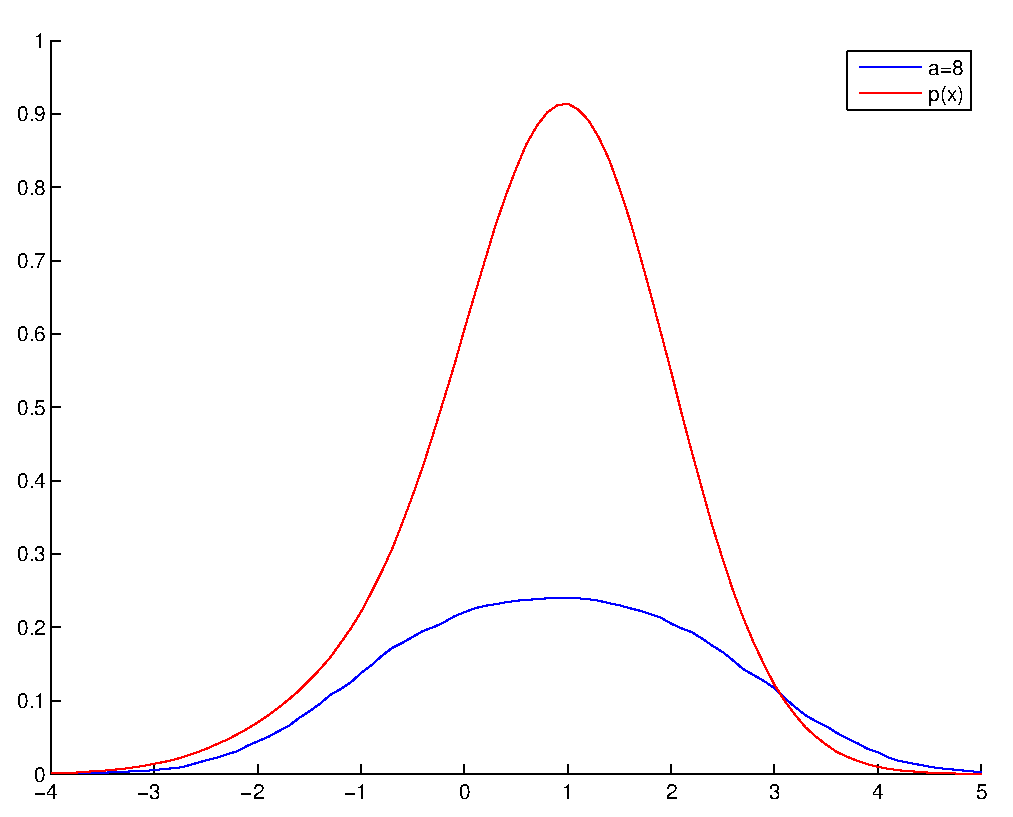
\includegraphics[width=2.1in]{8.eps}
\caption{a=8}
\end{minipage}
\begin{minipage}[t]{0.3\linewidth}
\centering
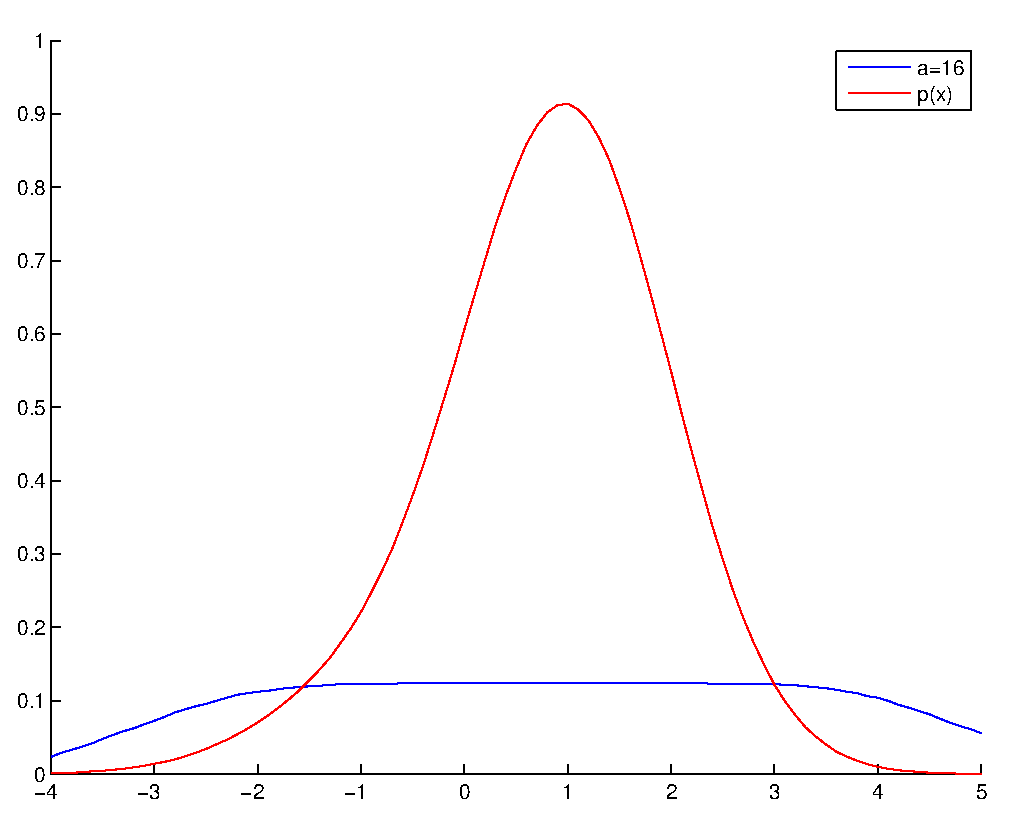
\includegraphics[width=2.1in]{16.eps}
\caption{a=16}
\end{minipage}
\end{figure}
(b)Derive how to compute $\epsilon(p_n)=\int[p_n(x)-p(x)]^2dx$ numerically.\\
\emph{\textbf{SOLUTION:}}\\
we can compute $\epsilon(p_n)$ by $\epsilon(p_n)\approx \sum_{i=1}^{T}[p_n(x_i)-p(x_i)]^2\Delta x_i$

(c)Demonstrate the expectation and variance of $\epsilon(p_n)$ w.r.t different $n$ and $a$ .

(d)With n given, how to choose optimal $a$ from above the empirical experiences?

(e)Substitute $h(x)$ in (a) with Gaussian window. Repeat (a)-(e).
\begin{figure}[!htbp]
\begin{minipage}[t]{0.3\linewidth}
\centering
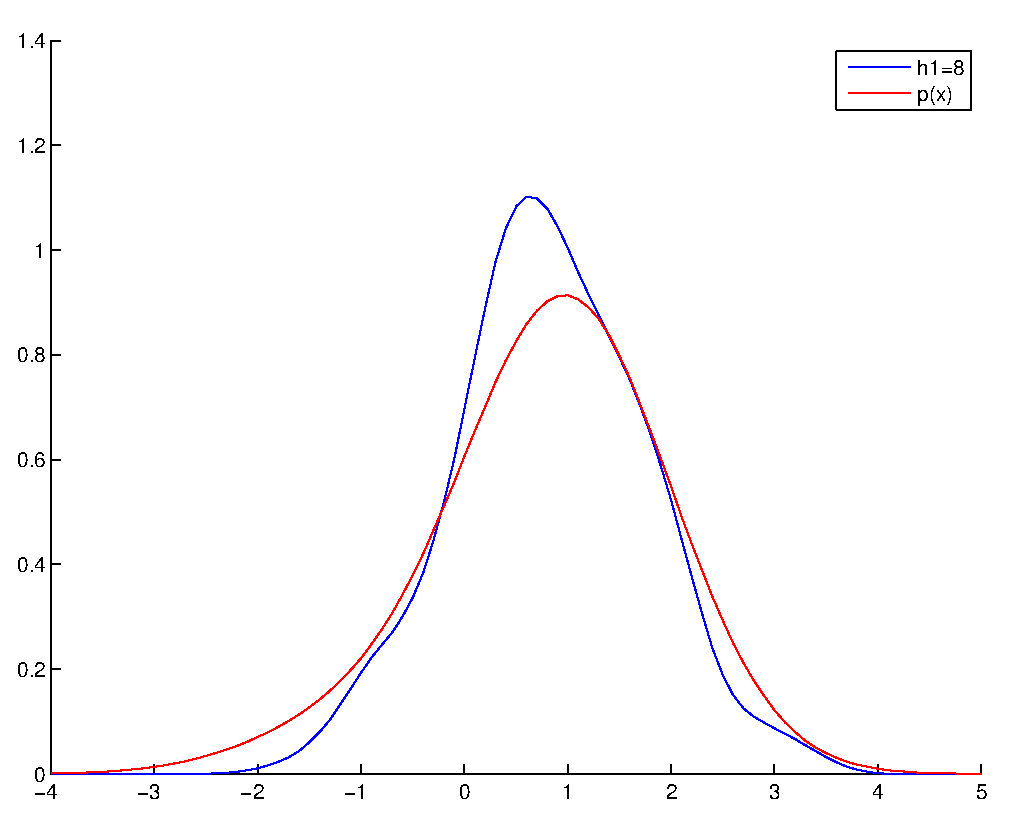
\includegraphics[width=2.1in]{g_8.eps}
\caption{$h_1=8$}
\end{minipage}%
\begin{minipage}[t]{0.3\linewidth}
\centering
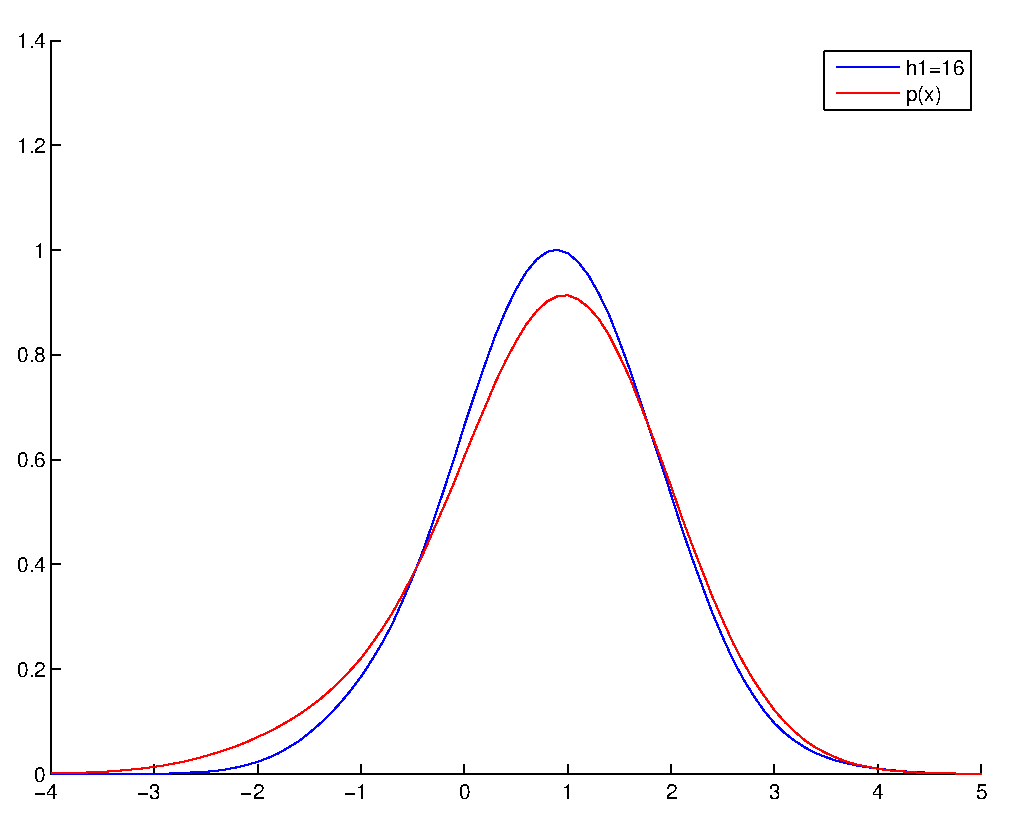
\includegraphics[width=2.1in]{g_16.eps}
\caption{$h_1=16$}
\end{minipage}
\begin{minipage}[t]{0.3\linewidth}
\centering
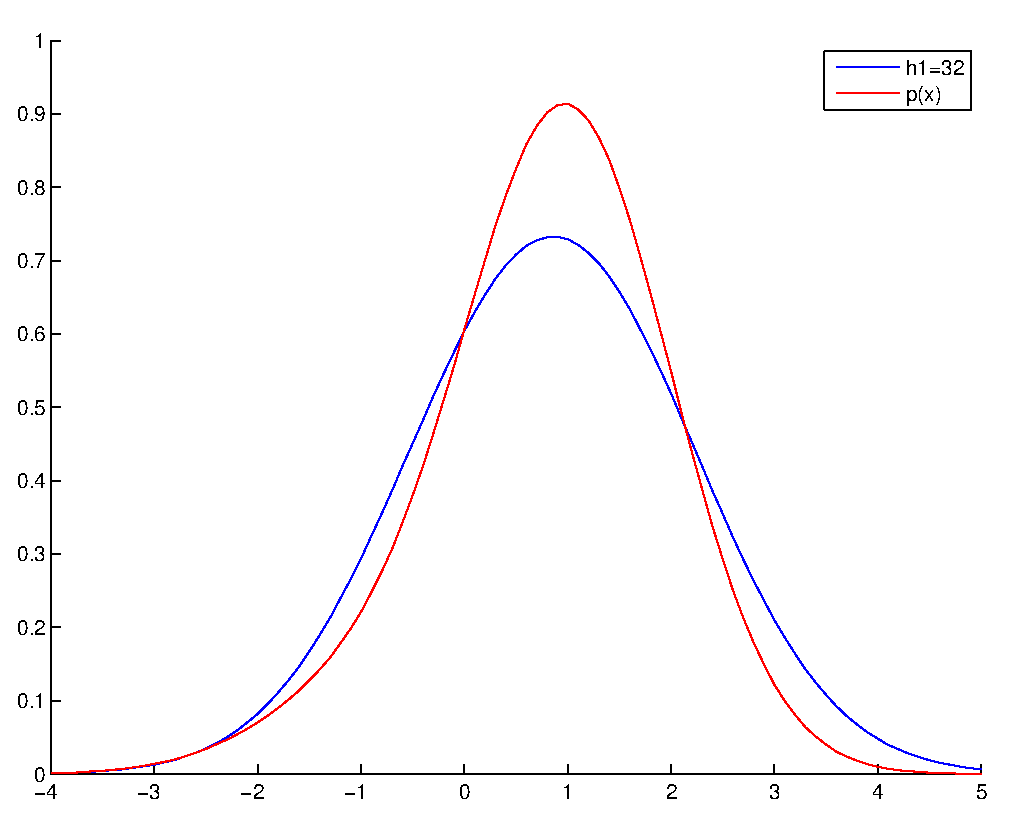
\includegraphics[width=2.1in]{g_32.eps}
\caption{$h_1=32$}
\end{minipage}
\end{figure}

(g)Try different window functions and parameters as many as you can. Which window
function/parameter is the best one? Demonstrate it numerically.\\
\emph{\textbf{SOLUTION:}}\\
From Figure 11 to Figure 13, we can see that Gaussian window functions is the best with smallest square error $\epsilon(p_n)$.\\
From Figure 14 to Figure 16, we can see that Gaussian windows functions with parameter $h_1=20$ is the best with smallest square error.
\begin{figure}[!htbp]
\begin{minipage}[t]{0.3\linewidth}
\centering
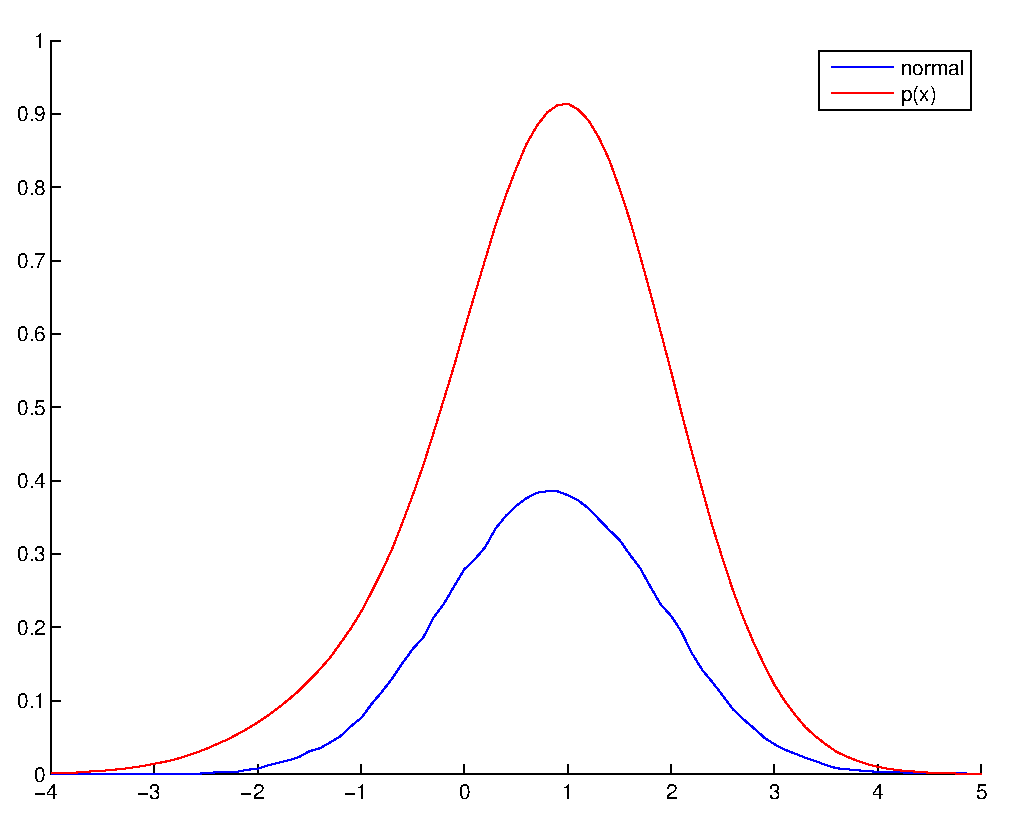
\includegraphics[width=2.1in]{normal.eps}
\caption{$error=0.5367$}
\end{minipage}%
\begin{minipage}[t]{0.3\linewidth}
\centering
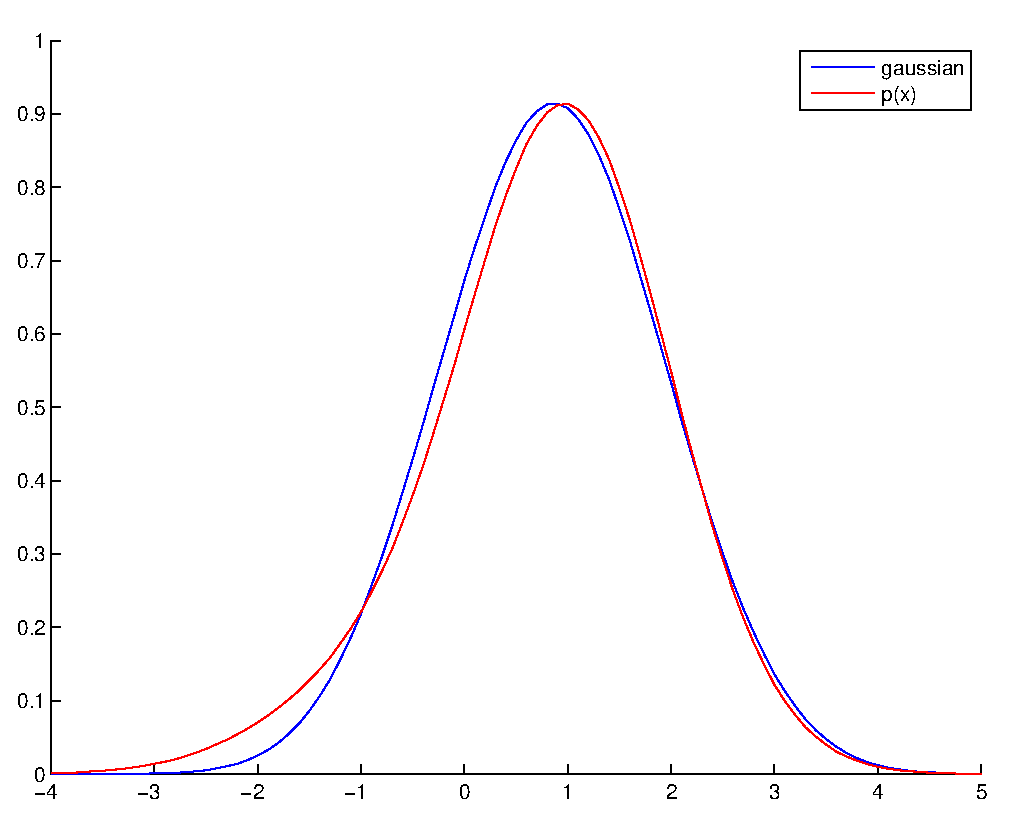
\includegraphics[width=2.1in]{gaussian.eps}
\caption{$error=0.0073$}
\end{minipage}
\begin{minipage}[t]{0.3\linewidth}
\centering
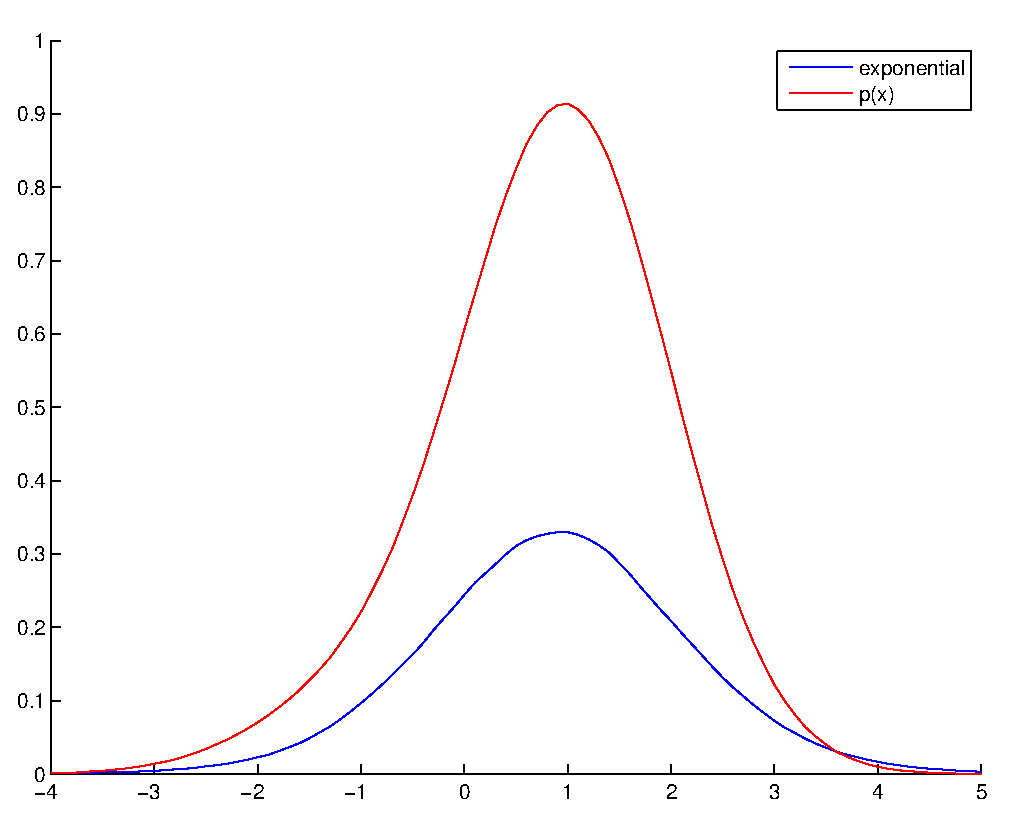
\includegraphics[width=2.1in]{exponential.eps}
\caption{$error=0.5887$}
\end{minipage}
\end{figure}

\begin{figure}[!htbp]
\begin{minipage}[t]{0.3\linewidth}
\centering
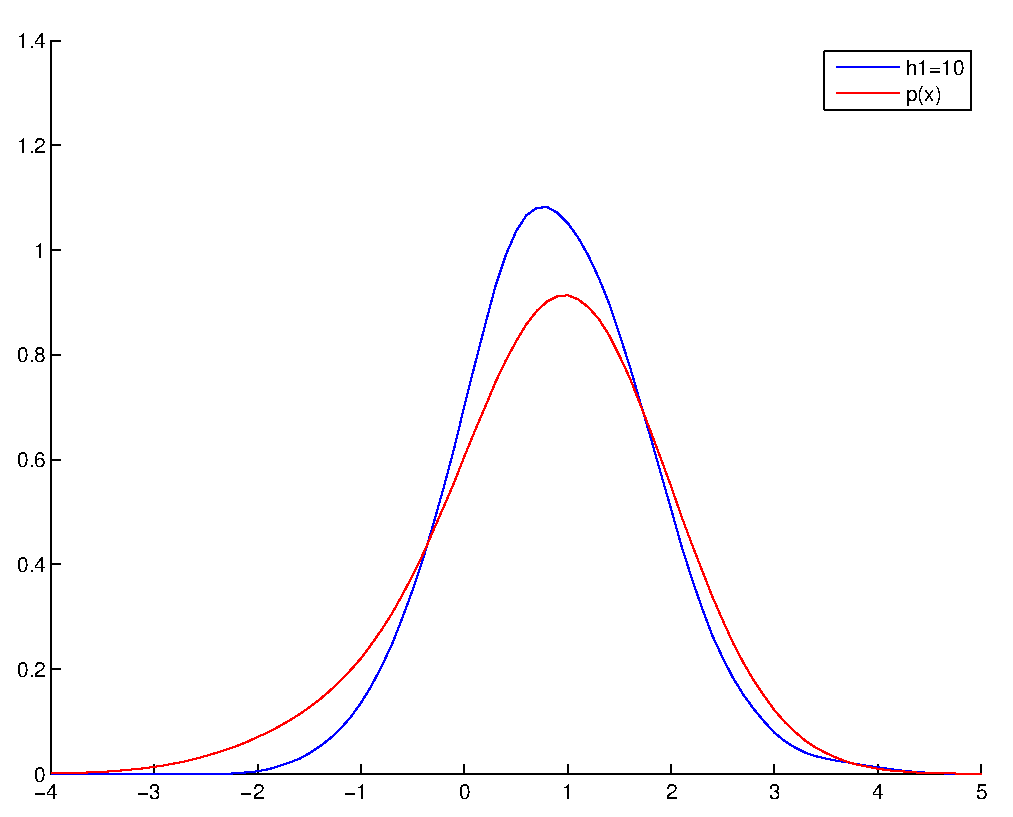
\includegraphics[width=2.1in]{gaussian10.eps}
\caption{$error=0.0561$}
\end{minipage}%
\begin{minipage}[t]{0.3\linewidth}
\centering
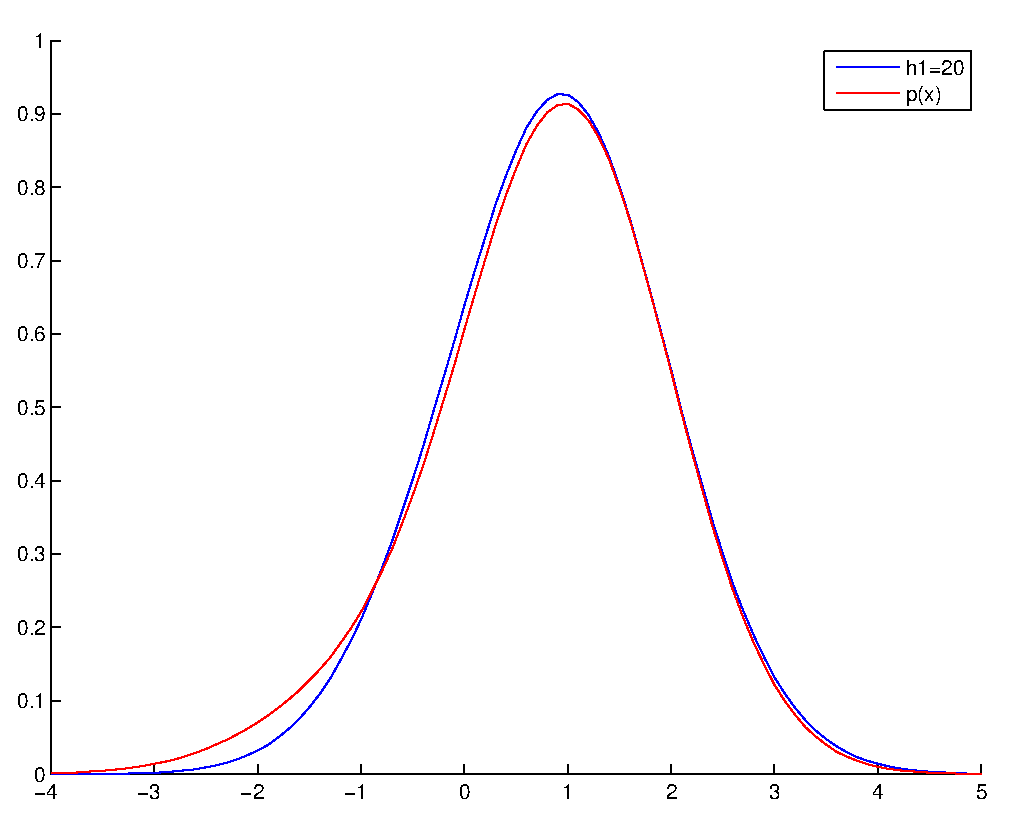
\includegraphics[width=2.1in]{gaussian20.eps}
\caption{$error=0.0057$}
\end{minipage}
\begin{minipage}[t]{0.3\linewidth}
\centering
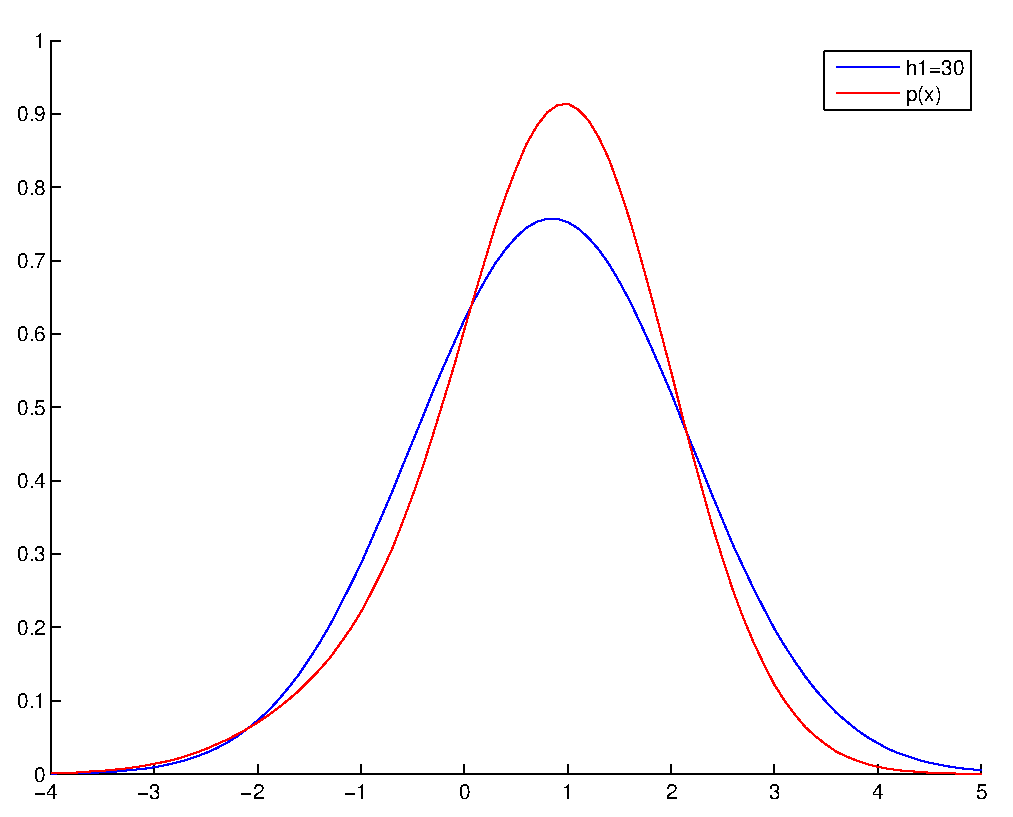
\includegraphics[width=2.1in]{gaussian30.eps}
\caption{$error=0.0381$}
\end{minipage}
\end{figure}

%%%%%%%%%%%%%%%%%%%%%%%%%%%%%%%%%%%%%%%%%%%%%%%%%%%%%%%%%%%%%%%%%%%%
% Reference
%%%%%%%%%%%%%%%%%%%%%%%%%%%%%%%%%%%%%%%%%%%%%%%%%%%%%%%%%%%%%%%%%%%%
%\begin{thebibliography}{1}

%\bibitem{BoydVandenberghe2004}
%S. Boyd and L. Vandenberghe, \emph{Convex Optimization}, Cambridge
%University Press, 2004.

%\end{thebibliography}
\end{document}
